\documentclass[11pt,a4j,twocolumn]{jarticle}

\usepackage[dvipdfmx]{graphicx}

\textheight=24cm \textwidth=16.5cm
\oddsidemargin=-8pt \topmargin=-25pt

\title{{\small A small talk on} Atomic Bombs}
\author{written by Ukichiro Nakaya,
published in October 1945\thanks{https://bit.ly/3xespbT}\\
translated by Takahiro Nakamura
}
\date{}

\begin{document}

\baselineskip=14.6pt

\maketitle

\noindent
On July 1937, the Marco Polo Bridge incident broke out in North China.
Pulled by an invisible force of history, 
the effect of the incident spread into Central China, 
in spite of the non-expansion policy of the Japanese government.
On October, Shanghai fell. As Japanese troops got close to the capital city Nanjing,
signs of world war became gradually apparent.

Just at that time, I wrote a short article entitled ``Bows and Guns."
It was published in ``Tokyo Aashi" on November 1937.
My clippings read:

\vspace{7.3pt}\noindent
``In a war between bows and guns, the latter would win.
But can you imagine that a new weapon of next era
degrades contemporary firearms just as guns degraded bows?

Firearms explode because of the chemical energy in molecules.
For example, energy in gunpowder comes out when its molecules combine,
and energy in dynamite comes out when its molecules decompose.
As you know, dynamite is much more energetic than gunpowder.
Naturally the next place to seek more energy is an atom,
because atomic energy is far greater than molecular energy.

Almost all of energy in an atom is stored in its nucleus.
Recently the mainstream of physics is directed to the study of nuclear decay.
Hopefully, for the benefit of humankind, nuclear energy will never be used to make weapons.
But if a certain country succeeded in making nuclear weapons,
then there would arise a turmoil which would swamp bows and guns.

In this regard, institutes for national defense may well have interests in
the research of atomic theory, which is the forefront of modern physics.
But one has to know that this research needs a lot of waste money.
For instance, at the Cavendish Laboratory in Cambridge,
it took ten years of hard work, as well as financial supports,
for sixty top-class physicists to get a first clue to the realization of nuclear energy."

\vspace{7.3pt}
When I wrote the short article, I didn't know about the nuclear fission of uranium,
which was used in the atomic bomb a few months ago.
Also the long-term experiments at the Cavendish Laboratory
just confirmed the mere possibility of artificial nuclear decay.
But looking back the modern history of scientific progress,
it seemed most natural to me to imagine that we look for
the next source of energy in atoms or in nuclei.

We line up such weapons in a row, as
gunpowder due to molecular combination,
followed by dynamite due to molecular decomposition,
followed by atomic bombs due to nuclear decay.
They are lined up only in our minds, 
but natural science dangerously makes them real.

A few years before the publication of the short article,
I told above things to some influential people in the ministry of national defense.
At that time in Japan, experiments in atomic physics were already begun
by Doctor Nishina in RIKEN and Professor Kikuchi in Osaka University.
So I infer that the ministry got advices from these institutes too.
But no one seriously adopted such advices, because there was no
prospect of realizing the weapon, even after several decades from then on.
This couldn't be helped, because it was the custom in our country
to define research as doing something that could be done when it was done.

However, a certain officer, who was then a head of a certain institute in navy,
showed a keen interest in this experiment. The officer said to me that
the naval institute would like to try the experiment.
I didn't have to respond, because
there were a lot of specialists in RIKEN and Osaka University. 
But I responded to the consultation because it was I who told
the ministry about nuclear weapons.

Looking back now, progress would have been much faster if
our research funds had been spent by those specialists
who had already begun experiments in atomic physics.
But circumstances then were such that research money couldn't
be transferred to other institutes if its amount was as large as tens of thousand yen.
In those days in that institute, such amount of money was considered
to be fairly large.

At that time in my laboratory, I was studying about electrical sparks,
using an instrument which was often used to study atoms.
Thus our experimental techniques were not so much unrelated to those of atomic physics.
So I had my assistant, Mr.\ T., leave my laboratory and go to the naval institute
to begin to work on atomic physics.

Of course it was totally impossible for Mr.\ T.\ alone to compete with 
top-class scientists who study hard with ample funds in the West.
So I responded to the officer on the following conditions.
We wouldn't contend with Western scientists, but just wait for their reports to be published.
Then we would select essential experiments from their reports, 
and try to reproduce their results in the laboratory of the naval institute.
This sounds rather servile, but would be regarded as success if
we could always follow their results, keeping a step behind them.
I proposed to set up such instruments in the laboratory, that
we might imitate them when they got nuclear energy for practical use.

The officer understood above things well, and agreed to my proposal at once.
We agreed to let Mr.\ T.\ set up necessary instruments,
and planned to send him to some institutes for atomic physics in the West.
The officer said that we could spend up to ten thousand yen for instruments.
What a tiny amount of money as compared to 
two billion dollars which America spent for the atomic bombs.
But at that time in our country,
ten thousand yen was an unprecedented amount of research money.

So far, so good. But just when Mr.\ T.\ joined the institute and began the research,
the head officer was told to move to another post.
It was when the Sino-Japanese war was becoming full-scale,
and the atmosphere in Japan was such that no one could afford to do research.
Thus the research in atomic physics was the first to be abandoned.
Mr.\ T.\ had to transform himself quickly into an assistant in metal physics
when he was told ``now that we are in a war regime, you must stop basic research,
and measure the thermal conductivity of gunmetals."
This was the end of the tale of ``my atomic bombs," a disappointingly short tale.

Reading the statements by the American government, I realized that
it was rather quixotic to attempt even to imitate their research on atomic bombs,
which was an unprecedented project in human history of science.
Mr.\ T.\ was, so to speak, timely dismissed from a role of Quixote.
Even if the head officer didn't move to another post,
it was surely impossible for us to make an atomic bomb,
no matter how much money we spent,
no matter how many researchers we employed,
and no matter how hard we worked.
The problem was not that we had no vein of uranium nor radium.
The problem was in the scientific levels of both influential people and the general public.

In 1938, Germany declared annexation of Austria, which plunged Europe into an abyss.
In 1939, Germany and Soviet Union concluded a nonaggression treaty.
In autumn of the year, Britain proclaimed war against Germany over the problem of Poland.
In 1940, German troops entered Paris, and German planes bombed London.
In 1941, German-Soviet war broke out, and America participated in the World War.
As the Sino-Japanese war expanded, no one in Japan could afford to do basic research. 

In the meantime, regardless of the World War, 
British and American scientists in atomic physics continued basic research.
For example, they measured the intensity of cosmic rays,
and measured the energy of radiations from nuclear decay.
Such experiments require large-scale equipments and huge amount of money.
The American government took care of such experiments, 
and constructed one equipment after another.
On participating in the World War, they first made an agreement with British government
about scientific research, so that some British scientists could go to America to collaborate.
A lot of Jewish scientists, who created German science and were persecuted in Germany,
also went to America and made great contributions to atomic physics.
When Hitler expelled such important scientists, he was cutting his own arms, so to speak.
In 1940, when Hitler entered Paris and confronted British Isles over the Strait of Dover,
the Fall of Berlin was already anticipated.
I wrote such an anticipation in ``Scientific Journals from Germany" which was 
published in ``Tokyo Asahi" on October 1940. I quote from it:

\vspace{7.3pt}\noindent
``My colleague physicist, who keeps up with new articles, said to me that
the quality of articles in German journals is getting low in recent years.
I agreed to him because I felt the same.
We agreed that America will exceed Germany in the academic world of physics,
if its rate of progress doesn't change.

Ardent admirers of German science may object that
the quality appears to get low because Germans keep important studies secret
and publish only trivial results. But if that's the case, one may smell
from their articles that they keep something secret.

Thus, basic research on science may look unimportant,
because there is no doubt about the high quality of
scientific weapons which Germans use in this World War.
On the contrary, we guess that Germans are now using up
legacies of great scientists whom Nazis expelled."

\vspace{7.3pt}
In fact, while Germans were using up their legacies,
Americans accumulated new knowledge.
They artificially disintegrated atoms in every element,
and studied the properties of radiations which came out from the disintegrations.
Their reports were published in ``Physical Review," which was
the main journal of the American Physical Society.
Every month, a lot of similar articles appeared in the journal,
in which they persistently reported their results for one atom after another.
Although enormous volume of articles appeared,
no one could tell exactly when nuclear energy would be put to practical use.

In 1940, however, a nuclear fission of uranium was somehow discovered to
be a terrible source of energy.
The news of the discovery reached Japan 
a year before the outbreak of the Pacific War, as I recall.
A decade had passed since Rutherford organized a team of
top-class physicists at the Cavendish Laboratory,
until the mainstream of physics was shifted from the theory of atomic structure
to that of nuclear structure.
Another decade had passed since Americans began investing huge resources
into the study of nuclear structure, until they got a glimpse of atomic power
from the discovery of the nuclear fission of uranium.

However, an atomic bomb was not at all completed by this discovery.
The discovery was like a dust particle that comprises a mountain.
Making an atomic bomb is to assemble a mountain from dusts.

Normally it would take, say, thirty years
to make an atomic bomb since the discovery of nuclear fission of uranium.
I didn't really think that an atomic bomb would be completed before the end of this World War.
Rumor said that Roosevelt noticed the nuclear fission of uranium
before the outbreak of the Pacific War, and cooperated with Churchill
to mobilize physicists from both countries in order to create new weapons.
I slighted the rumor, because I never thought that they could create new weapons
in a few years, no matter how many resources they invested.

It was not until the atomic bombs were dropped in Japan that I understood how big this World War was.
Who could imagine that two billion dollars and sixty-five thousand engineers were secretly
invested for four years into a project which was not guaranteed to succeed?
Such a big project would be impossible in our country, unless a success was guaranteed.

Here is an anecdote. During this World War,
a committee on the research of nuclear decay was organized in our country too.
A competent physicist, who was a member of the committee,
visited a government office and met an influential officer.
The officer asked the physicist what was necessary for the research.
The physicist replied cynically that a brass bar was necessary.
This sounds like a joke. But, judging from my experience, I don't think this is a fiction.
The physicist demanded a brass bar because he knew that
our government would never understand the necessity of basic research,
which needs a lot of waste money. 
He was too cynical to demand what he really needed, I suppose.
What we scientists really need is non-scientist's understanding
about the importance of basic research on science.

To reconstruct Japan after the war, national resources must be built up
on scientific grounds, and this is possible only if
the general public understand the value of scientific methods.
One must not misunderstand that our aim is to create new weapons
which are stronger than theirs.
It was rather fortunate that we Japanese were unable to make an atomic bomb during the war.
I wrote ``hopefully, nuclear energy will never be used to make weapons"
in my article eight years ago. Now I hope so too.
When I saw the cruelty of the atomic bombs, 
I felt that we humankind have gone too far on the way of scientific progress.

On this Earth, nuclear energy had been tightly locked up in atoms,
since the creation of the Solar System.
The energy comes out only on the occasion of nucleosynthesis during a supernova explosion
which occurs in the distant universe.
We humankind had unlocked the energy, and opened the Pandora's box, so to speak.
There is a good reason to fear that we had already taken
a first step toward the extinction of humankind.
When atomic bombs are mass-produced as firearms in the future,
the first atomic bomb that was used in the war will properly be compared to a matchlock.
Just as matchlocks evolved to guns, atomic bombs will keep on evolving.

A new invention is generally difficult because no one knows whether
the invention is possible at all. Once someone shows that an invention is ever possible,
its difficulty is reduced in half, say.
It won't be long until several countries catch up with America,
and produce various types of atomic bombs.
These bombs will be loaded on long-range missiles, 
so that they can fly to everywhere around the world.
May we stop thinking about the final day of humankind.

The atomic bombs reminded me of a Western philosopher's saying,
``science does not always contribute to happiness of humankind."
But the word ``science" in the above saying means technology rather than science.
Intrinsically, science means a quest for the truth, motivated by adoration
toward the mysteries of nature.
Evil aspects of ``science" have been too conspicuous in modern times.
I hope that its intrinsic aspects will be more emphasized in postwar times.
I am sure that this hope is shared by many people not only in our country but also in America.

\vfill
\noindent
\centerline{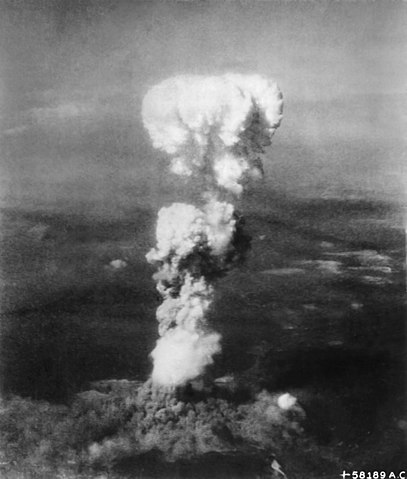
\includegraphics[width=\columnwidth,bb=0 0 408 1]{hiroshima.jpg}}

\end{document}